\chapter{Grundlagen}
\label{cha:grundlagen}

\section{Historie von Identitätsmanagementsystemen und deren Status Quo}
Die Historie von Identitätsmanagementsystemen ist geprägt von verschiedenen Ansätzen, darunter die zentralisierte Identität (centralized Identity), die föderierte Identität (federated Identity), die nutzerzentrierte Identität (user-centric Identity) und die selbstbestimmte Identität (self-sovereign Identity). Die angegeben Identitätssysteme schließen sich nicht gegenseitig aus und vor allem die dezentrale Identität wird in modernen dezentralen Identitätsmanagementsystemen in Kombination mit seinen Vorgängern implementiert.

Zentralisierte Identitätssysteme waren lange Zeit vorherrschend, bei denen Identitätsinformationen in zentralen Datenbanken gespeichert wurden. Organisationen und Behörden kontrollierten den Zugriff auf diese Daten und verwalteten die Identitäten der Benutzer. Dabei authentifiziert sich ein Nutzer mit einer Nutzeridentifikation und einem Password.  Dieser Ansatz führte jedoch zu Fragmentierung, Ineffizienz und möglichen Sicherheitsrisiken, wenn Nutzer nicht unterschiedliche Login-Daten für jeden Online-Dienst verwenden.

Mit der Einführung der föderierten Identitätssysteme wurde versucht, diese Probleme zu lösen. Hierbei können Benutzer über einen Identitätsanbieter, wie beispielsweise ein soziales Netzwerk oder ein Unternehmenskonto, auf verschiedene Dienste zugreifen. Der Identitätsanbieter fungiert als Vermittler und ermöglicht den nahtlosen Zugriff, ohne dass Benutzer separate Anmeldeinformationen für jeden Dienst bereitstellen müssen. Das Konzept hinter der föderierten Identität lautet \textsl{Single-Sign-On (SSO)}. Dabei gibt der Nutzer pro Sitzung seine Login-Daten einem \textsl{Identitätsanbieter} (Google, Facebook, etc), welcher im Gegenzug ein signiertes Token ausstellt, welches für kommende Logins verwendet wird. Die dabei verwendeten Technologien sind beispielsweise \textsl{SAML} \cite{ID12} oder \textsl{OpenID Connect} \cite{ID13}.

Die nutzerzentrierte Identität rückt den Benutzer in den Mittelpunkt des Identitätsmanagements. Bei diesem Ansatz behalten Benutzer die Kontrolle über ihre Identitätsdaten und können sie in einer sicheren Umgebung speichern. Sie können ihre Daten selektiv freigeben und verwalten, was zu mehr Privatsphäre und Kontrolle führt. Eine Implementierung hierfür ist BrowserID\cite{ID14}. Durchgesetzt hat sich diese Technologie jedoch nicht, da es an Akzeptanz und Integration durch Webseiten mangelte.

Die selbstbestimmte Identität oder Self-Sovereign Identity (SSI) stellt den neuesten Ansatz dar. Bei SSI behalten Benutzer die vollständige Kontrolle über ihre Identitätsdaten, indem sie kryptografische Schlüssel verwenden. Die Identitätsdaten werden dezentralisiert und auf der Blockchain oder anderen verteilten Systemen gespeichert. Benutzer können selektiv Informationen freigeben und verifizieren, wodurch ihre Privatsphäre und Sicherheit gestärkt werden.

\section{Self-Sovereign-Identity}

\subsection{Das Konzept hinter SSI}	
	Das Konzept der Self-Sovereign Identity \cite{SOV1} basiert auf den folgenden Prin
	
	zipien:
	
	\begin{enumerate}
		\item Benutzerkontrolle: Der Benutzer hat die ultimative Kontrolle über seine Identität und die damit verbundenen Daten. Der Benutzer kann bestimmen, welche Informationen er teilen möchte, mit wem und zu welchen Bedingungen.
		
		\item Dezentralisierung: Die Identitätsdaten sind nicht an eine zentrale Institution oder Datenbank gebunden. Stattdessen werden sie dezentral auf verschiedenen Plattformen, Geräten oder Blockchains gespeichert. Der Benutzer hat die Möglichkeit, seine Identitätsdaten an einem sicheren Ort seiner Wahl zu speichern.
		
		\item Interoperabilität: SSI strebt nach Interoperabilität zwischen verschiedenen Identitätsplattformen und -systemen. Das bedeutet, dass Identitätsdaten zwischen verschiedenen Diensten und Organisationen ausgetauscht und verifiziert werden können, ohne dass eine zentrale Instanz benötigt wird.
		
		\item Vertrauensmodelle: SSI nutzt kryptografische Technologien, wie digitale Signaturen und Blockchains, um die Integrität und Vertrauenswürdigkeit von Identitätsdaten zu gewährleisten. Es ermöglicht auch das Prinzip der Verifizierung von Informationen, bei dem die Authentizität bestimmter Daten von anderen Parteien bestätigt werden kann.
		
		\item Datenschutz und Privatsphäre: SSI legt großen Wert auf Datenschutz und Privatsphäre. Der Benutzer hat die Kontrolle darüber, welche Informationen freigegeben werden und welche nicht. Es ermöglicht auch selektive Offenlegung, bei der nur die notwendigen Informationen für einen bestimmten Zweck oder Kontext offengelegt werden.
	\end{enumerate}
	
	Das Ziel von Self-Sovereign Identity ist es, die Verwaltung von Identitätsdaten für Benutzer transparenter, sicherer und benutzerzentrierter zu gestalten. Es bietet die Möglichkeit, Identitätsinformationen nahtlos zwischen verschiedenen Diensten und Organisationen zu nutzen, während die Kontrolle über die eigenen Daten in den Händen des Benutzers bleibt.
	


\subsection{Identität}
Im Kontext der Self-Sovereign Identity (SSI) gibt es verschiedene Konzepte, die verschiedene Aspekte der Identität und Kontrolle berücksichtigen. Zwei solcher Konzepte sind die \textsl{Weak/Nym Identity} und die \textsl{Partial/Strong Identity}.

Die Weak/Nym Identity bezieht sich auf eine Identität, die nur begrenzte Informationen über den Benutzer enthält. Bei dieser Identität wird bewusst darauf verzichtet, persönliche Informationen oder Details preiszugeben, die zur Identifizierung des Benutzers verwendet werden könnten. Stattdessen wird ein Pseudonym oder ein Alias verwendet, um die Privatsphäre des Benutzers zu schützen. Die Weak/Nym Identity ermöglicht es dem Benutzer, Transaktionen durchzuführen und Dienste zu nutzen, ohne seine wahre Identität preiszugeben.

Im Gegensatz dazu bezieht sich die Partial/Strong Identity auf eine Identität, die umfassendere Informationen über den Benutzer enthält. Diese Identität kann persönliche Daten wie Name, Adresse, Geburtsdatum und andere relevante Informationen enthalten. Die Partial/Strong Identity ermöglicht eine genauere Identifizierung und Authentifizierung des Benutzers, was in einigen Situationen erforderlich sein kann, beispielsweise bei behördlichen Anforderungen oder bei Zugang zu sensiblen Diensten. Die Partial/Strong Identity erfordert eine sorgfältige Verwaltung der Identitätsdaten, um sicherzustellen, dass sie sicher und geschützt bleiben.

Beide Identitätskonzepte haben ihre eigenen Vor- und Nachteile in Bezug auf Datenschutz, Sicherheit und Benutzerkontrolle. Die Entscheidung für eine bestimmte Identität hängt von den individuellen Anforderungen, dem Kontext und den Präferenzen des Benutzers ab. SSI strebt jedoch nach Flexibilität und Wahlfreiheit für Benutzer, um die Identität zu wählen, die ihren Bedürfnissen am besten entspricht und gleichzeitig die Sicherheit und den Schutz ihrer Daten gewährleistet.

In den folgenden Kapiteln wird in der Konzeption und Implementierung ein Minimum an Daten preisgegeben, also eine schwache Identität. Jedoch werden auch Anwendungsfälle berücksichtigt, wo Informationen zur Identität benötigt werden.

\subsection{Technische Grundlagen}
Um das Konzept der Self-Sovereign Identity (SSI) aus technologischer Sicht zu verstehen und anzuwenden, sind folgende Kernkonzepte erforderlich \cite{ID16} \cite{ID17}:

\begin{enumerate}
	\item Trust-Registries: Diese dienen als gemeinsame und vertrauenswürdige Aufzeichnung bestimmter Informationen. Mit anderen Worten fungieren sie als 'Vertrauensebene' und 'einzige Quelle der Wahrheit'. Eine mögliche Realisierung einer Trust-Registry ist ein dezentraler Speicher (Distributed Ledger), der alle Aktivitäten in Transaktionen speichert.
	
	\item Kryptografische Schlüssel: Diese übertragen die Kontrolle über digitale Identitäten und ermöglichen grundlegende Funktionen wie Verschlüsselung und Authentifizierung. Hierbei handelt es sich um klassische private/öffentliche Schlüsselpaare, die im Falle von der Bitcoin-Blockchain 48 Byte / 256 Bit lang sind \cite{ID15} und dem Verschlüsseln/Entschlüsseln/Signieren von Daten dienen.
	
	\item Dezentrale Identifikatoren (DIDs): DIDs sind globale und einzigartige Identifikatoren, die keine zentralen Register zur Speicherung benötigen. Sie unterscheiden sich zu UUIDs in dem Sinne, dass DIDs auf sog. DID-Documents zurückzuführen sind und mit kryptographischen Mechanismen Eigentumsverhältnisse zeigen. DID's sind aufgebaut wie folgt:\\
	\textsl{"did:" \textlangle Methodenname\textrangle ":" \textlangle methodenspefizische-ID\textrangle\\
	Beispiel:"did:btcr:abcd-1234-wxyz:789"}\\
	Dabei zeigt ein DID immer auf ein DID-Dokument, welches im JSON-Format Metadaten wie öffentliche Schlüssel oder Authentifizierungsmethoden beinhaltet.
	
	Ein DID-Document sieht wie folgt aus:
	\begin{lstlisting}[language=json,firstnumber=1]	
{
	"id": "did:ion:EiClkZMDxPKqC9c-umQfTkR8vvZ9JPhl_xLDI9Nfk38w5w",
	"@context": [
	"https://www.w3.org/ns/did/v1",
	{
		"@base": "did:ion:EiClkZMDxPKqC9c-umQfTkR8vvZ9JPhl_xLDI9Nfk38w5w"
	}
	],
	"service": [
	{
		"id": "#linkedin",
		"type": "linkedin",
		"serviceEndpoint": "linkedin.com/in/henry-tsai-6b884014"
	},
	{
		"id": "#github",
		"type": "github",
		"serviceEndpoint": "github.com/thehenrytsai"
	}
	],
	"verificationMethod": [
	{
		"id": "#someKeyId",
		"controller": "did:ion:EiClkZMDxPKqC9c-umQfTkR8vvZ9JPhl_xLDI9Nfk38w5w",
		"type": "EcdsaSecp256k1VerificationKey2019",
		"publicKeyJwk": {
			"kty": "EC",
			"crv": "secp256k1",
			"x": "WfY7Px6AgH6x-_dgAoRbg8weYRJA36ON-gQiFnETrqw",
			"y": "IzFx3BUGztK0cyDStiunXbrZYYTtKbOUzx16SUK0sAY"
		}
	}
	],
	"authentication": [
	"#someKeyId"
	]
}
	\end{lstlisting}
	
	Es ist zu erkennen, dass dieses DID-Document festlegt für welche Services dieses Dokument die Authentifikation definiert (in diesem Falle LinkedIn und Github). Unter 'verificationMethod' wird der Typ 'EcdsaSecp256k1VerificationKey2019' angegeben, was einer Public-Key-Authentifikation entspricht, welche Elliptic-Curve-Kryptografie verwendet.
	
	\item Verifizierbare Nachweise (VCs): VCs sind digitale Identitätsdokumente, die von jedem auf ihre Gültigkeit, Integrität, Authentizität und Herkunft hin überprüft werden können. Sie beinhalten sog. \textsl{Claims}, also Informationen/Behauptungen über die Entität (beispielsweise den Namen, Geburtsdatum, etc.). Wichtig ist, dass VCs aus Datenschutz- und Compliance-Gründen niemals auf einer Blockchain gespeichert werden. Ein VC kann wie folgt aussehen:
	
	\begin{lstlisting}[language=json,firstnumber=1]
{
	"@context": [],
	"id": "e9ea3429-b32f-44ad-b481-b9929370bb90",
	"type": [ "VerifiableCredential", "ExampleCredential" ],
	"issuer": { "id": "did:btcr:2d28bb79-87a9-4224-8c63-d28b29716b67" },
	"issuanceDate": "2022-01-01T00:00:00Z",
	"credentialSubject": {
		"id": "did:example:7564cb9c-165c-4857-a887-bfc2460af867",
		"birth_date": "1970-01-01"
	},
	"expirationDate": "2023-01-01T00:00:00Z",
	"proof": {<SignatureOfIssuer>}
}
	\end{lstlisting}
	
	Es ist zu erkennen, dass in dem VC unter anderem Claims ('credentialSubject' genannt) enthalten sind (in diesem Falle das Geburtsdatum), der Issuer des VC, ein Auslaufdatum und ein 'Proof', also eine digitale Signatur des Issuer's, um die Integrität des VC's zu überprüfen.
	
	\item Wallets: Wallets speichern unsere Schlüssel und VCs und ermöglichen die Verwaltung und Nutzung unserer digitalen Identitäten und Daten über benutzerfreundliche Anwendungen.
\end{enumerate}

Diese Kernkonzepte bilden die Grundlage der SSI-Technologie. Sie ermöglichen es Einzelpersonen, die Kontrolle über ihre digitalen Identitäten zu haben, verifizierbare Nachweise sicher zu teilen und vertrauenswürdige Interaktionen mit anderen durchzuführen.


Das grobe Zusammenspiel der Komponenten sieht dabei wie folgt aus:

\begin{figure}[h]
	\centering
	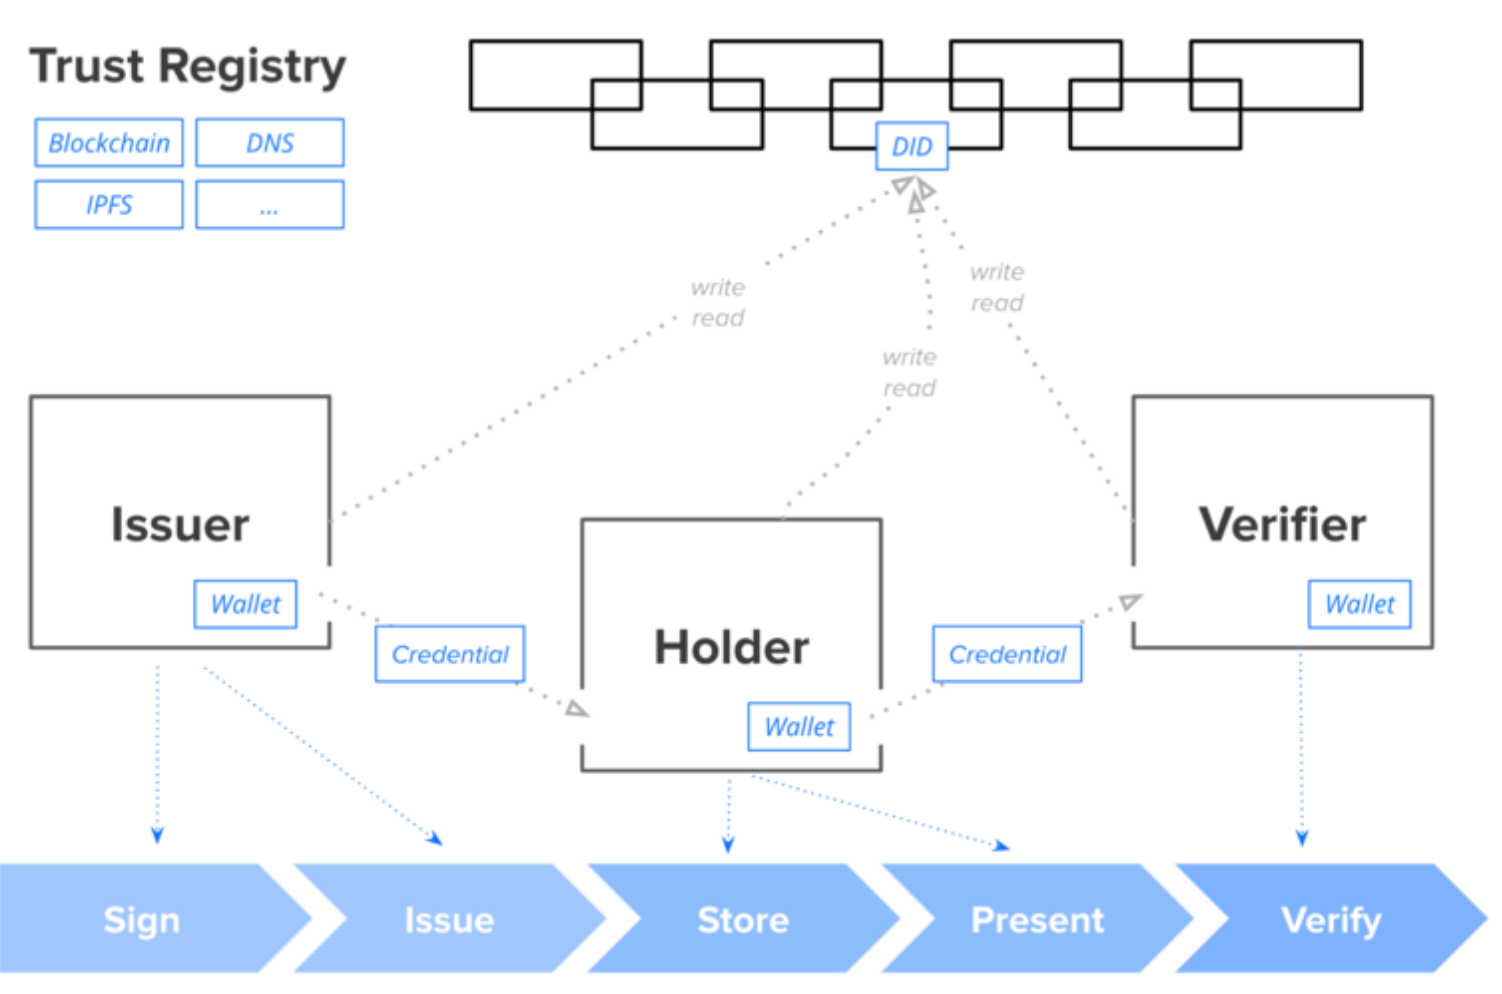
\includegraphics[scale=0.3]{media/zusammenspiel.png}
	\caption{Zusammenspiel von Issuer, Holder und Verifier \cite{ID62}}
	\label{fig:meine-grafik}
\end{figure}

Es ist zu erkennen, dass sowohl Issuer, Holder und Verifier Eigentümer von einem Wallet sind. Der Issuer (beispielsweise eine Bank) stellt VC's aus, die der Holder (Beispielsweise eine Privatperson) in seinem Wallet speichert. Muss sich dieser nun ausweisen, so reicht er dem Verifier (Beispielsweise der Arbeitgeber) eine VC-Representation ein. Diese VC-Representation (oder auch Verifiable Presentation \textsl{VP} genannt) beinhaltet in der Regel ein VC, kann jedoch in komplexeren Szenarien mehrere VC's enthalten. Zudem sind alle Akteure (insbesondere der Verifier) in der Lage die Authentizität des VP zu überprüfen.\\

Issuer, Holder und Verifier können jeweils alle drei Rollen annehmen, besitzen eine DID und sind DID-Subjects. Folgende Zusammenhänge existieren zwischen dem DID-Subject, DID, DID-URL, DID-Controller, DID-Document und der Verifiable Data Registry:

\begin{figure}[H]
	\centering
	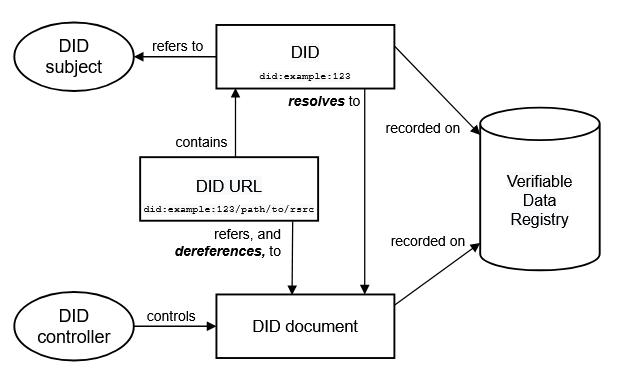
\includegraphics[scale=0.9]{media/DID.PNG}
	\caption{DID-Objekte und deren Zusammenhänge \cite{ID18}}
	\label{fig:meine-grafik}
\end{figure}

Die DID-URL beinhaltet die DID und erweitert die Syntax um die URI-Komponenten wie Pfade oder Anfrage-Parameter. Sowohl DID's als auch DID-Documents werden auf einem Verifiable Data Registry persistiert. Diese werden beispielsweise als Datenbanken oder dezentrale Dateisysteme realisiert. In diesem Kontext sind jedoch distributed Ledger die Speicher der Wahl. Das DID-Dokument wird durch die DID-URL (de-)referenziert und durch die DID auf sich verwiesen. Der DID-Controller ist die Entität, die das DID-Document modifizieren kann. In der Regel ist diese Entität das DID-Subject der DID, es kann jedoch auch
 ein oder mehrere andere DID-Subjekte sein.


\section{Politik, Recht und Ethik in Bezug auf SSI}

\subsection{Politik}
Aus politischer Sicht spielt SSI eine wichtige Rolle, da das Potential besteht das Monopol des Staates in Bezug auf die Ausstellung, Aufrechterhaltung und Entzug von Ausweisdokumenten zu verlieren. Durch die Einführung von digitalen Entitäten - mit denen man sich auch in der analogen Welt ausweisen könnte - können staatliche Institutionen nicht mehr uneingeschränkt über den genannten Prozess verfügen. Betroffen sein können unter anderem die Digitalisierung der Grenzkontrollen oder das Migrationsmanagement, indem Pässe, Visa und ähnliche Dokumente als VC zur Verfügung gestellt werden. \\
Eine weitere Auswirkung ist, dass durch SSI das aktuelle Monopol im Identitätsmanagement von Unternehmen wie Meta (Facebook) und Google durch föderierte Identitätsmanagementsysteme abgelöst wird. Dadurch haben letztere Unternehmen nicht mehr die Kontrolle über die Daten ihrer Nutzer, was auch monetäre Auswirkungen hat. Die zuvor für Marketingzwecke verwendeten Daten stehen demnach nicht mehr zu Verfügung für personalisierte Werbung und Ähnlichem.\\
Insgesamt hat SSI das Potenzial, das bestehende Identitätsmanagement-System zu revolutionieren und die Kontrolle über digitale Identitäten in die Hände der Nutzer zu legen. Dies wirkt sich auf verschiedene Bereiche aus, darunter die Politik, das Monopol des Staates, die Digitalisierung von Grenzkontrollen und die Monetarisierung von Daten.

\subsection{Recht}
Die Einführung von SSI wirft auch rechtliche Fragen und Aspekte auf. Eine zentrale Frage betrifft die rechtliche Anerkennung von digitalen Identitäten und die damit verbundenen Rechte und Pflichten. Da SSI die traditionelle Vorstellung von staatlich ausgestellten Ausweisdokumenten und Identitätsnachweisen herausfordert, müssen rechtliche Rahmenbedingungen geschaffen werden, um die Verwendung und den Schutz digitaler Identitäten zu regeln. Dies könnte die Festlegung von Standards für digitale Identitäten, Datenschutzbestimmungen, Haftungsfragen und den Zugriff auf und die Verwaltung von persönlichen Daten umfassen. Zudem muss auch geklärt werden, wie SSI in bestehende Rechtssysteme und -strukturen integriert werden kann, beispielsweise in Bezug auf Verträge, Gerichtsverfahren oder behördliche Angelegenheiten. Die rechtlichen Aspekte von SSI sind daher von großer Bedeutung, um die rechtliche Sicherheit, den Schutz der Privatsphäre und die Gewährleistung der Rechte und Pflichten aller beteiligten Parteien zu gewährleisten.\\
Weitere zu beachtende Aspekte sind die juristische Verantwortlichkeit oder Datenschutz. Vor allem Ersteres spielt eine Rolle, wenn es sich um die Verwendung von Identitätsinformationen, Identitätsdiebstahl oder Fälschungsversuchen handelt. Zweiteres ist relevant in Bezug auf die rechtlichen Anforderungen die mit Datenverwaltung einhergehen.

\subsection{Ethik}
Auch auf ethnischer Sicht zeigt sich die Relevanz von SSI. Gerade das Konzept der Dezentralisierung und die Tatsache, dass keine Instanz mehr Macht über die Identitäten hat als andere wirft ethnische Fragestellungen auf. In \cite{ID17} beschreibt Ishmaev das Paradoxon, dass einerseits SSI zuletzt genannte Eigenschaften fordert, jedoch andererseits verschiedene Levels an 'Vertrauen' an Entitäten in der analogen Welt existieren. So sind beispielsweise Dokumente, die von einer staatlichen Autorität zugewiesen werden bedeutender als das Sportabzeichen für Grundschüler. Dieser Zustand wird in dem SSI-Konzept jedoch nicht berücksichtigt und zeigt den Kompromiss, den SSI-Identitätsmanagementsysteme implementieren müssen.\\
Ein weiterer problematischer Aspekt, ist die von Ishmaev genannte Tatsache, dass die Macht über die Freigabe der Daten zwar bei dem Nutzer liegt, die Macht über die Nutzung eines Dienstes liegt jedoch weiterhin bei dem Anbieter. So kann ein Großkonzern für die Nutzung eines Dienstes eine unmoralische Menge an Informationen fordern. Dadurch wird klar, dass weiterhin eine problematische Machtrelation existiert.\\

Ein weiterer Punkt ist die Diskrepanz zwischen SSI im sozialen und im technischen Kontext. SSI-Systeme unterscheiden nicht zwischen den handelnden Entitäten, ob es sich um Privatpersonen, Institutionen oder - im Rahmen von Internet-of-Things - Hardware handelt. Gerade dadurch weißt die Interpretation von 'Vertrauen' in sozialen oder cybersecurity Bereich Unterschiede auf. Es gibt eine Vielzahl an Definitionen für "Vertrauen", wobei diese meist in Abhängigkeit zu dem Kontext stehen, in dem sie verwendet werden. Eine allgemeine Definition wurde von McKnight und Chervany (1996) festgelegt: Vertrauen ist der Grad zu welchem eine Partei einwilligt abhängig zu etwas oder jemanden in einer Situation zu sein mit einem Gefühl von Sicherheit. Hierbei werden explizit und implizit folgende drei Bestandteile von Vertrauen dargestellt \cite{ID24}:
\begin{itemize}
	\item Abhängigkeiten zwischen Parteien
	\item Zuverlässigkeit einer Partei
	\item Risiko, dass eine Partei nicht wie erwartet agiert
\end{itemize}
Alle diese drei Charakteristika unterscheiden sich, je nachdem ob es sich um IoT-Geräte, Software oder Menschen handelt. 


\section{Merkmale und Vorteile von DLT}
Distributed Ledger ist - wie der Titel bereits beschreibt - eine , für diese Arbeit, bedeutende Technologie. Dabei sind folgende Merkmale und Vorteile der DTL relevant \cite{ID19}:
\begin{itemize}
	\item DLT ermöglicht das Betreiben einer hochverfügbaren Datenbank (eines 'Ledgers'), da nicht eine zentrale Instanz für die Verfügbarkeit verantwortlich ist, sondern die Gesamtheit der Knoten in dem Netzwerk.
	
	\item Ebenso ermöglicht die Dezentralität des DLT eine verteilte Speicherung und Verarbeitung.
	
	\item Manipulationsresistenz wird durch kryptographische Verfahren innerhalb der Blockchain sichergestellt. Im Fall  der Blockchain sind diese in der Regel asymmetrische Verfahren, was bedeutet, dass private/öffentliche Schlüssel zum Ent- oder Verschlüsseln der Daten verwendet werden, wobei 'Integer Factorization', "Discrete Logarithm' oder 'Elliptic Curves' verwendet werden können \cite{ID23}
	
	\item Zensurresistenz kann gewährleistet, indem beispielsweise alle Knoten die gleichen Berechtigungen haben und somit keine machthabende Instanz existiert. Alle Teilnehmer im Netzwerk werden als Knoten (Nodes) bezeichnet und besitzen jeweils eine lokale Kopie des Ledgers. Änderungen werden nun auf der Kopie ausgeführt und im Anschluss in dem Netzwerk synchronisiert. Das Netzwerk gilt als 'untrustworthy' (nicht vertrauenswürdig), wenn willkürliche einzelne Knoten sog. 'Byzantine-Failures' \cite{ID20} \cite{ID21} erzeugen können. Dies bedeutet, dass versucht wird beliebig falsches Verhalten im System zu erzeugen (unauthentische Daten, Zusammensturz des Systems, etc). Der Resistenzgrad des Netzwerks gegenüber diesen Angriffen wird als 'Byzantine-Toleranz' bezeichnet und wird in der Regel durch Abstimmungen im Netzwerk (Beispielsweise Konsensus-Algorithmen) verhindert. Beispiele im Blockchain-Kontext sind 'Proof-of-Work' oder "Proof-of-Stake' \cite{ID22} angewandte Algorithmen.
	
	\item Möglichkeit zur 'Demokratisierung' von Daten: Durch DLT kann ermöglicht werden, dass Individuen und/oder Organisationen kooperativ Kontrolle über Daten ausüben
	
\end{itemize}

\section{Anwendung von DLT im Bereich der digitalen Identität}
Die oben genannten Eigenschaften sind für das Betreiben eines Identitätsmanagementsystems optimal, da diese hochverfügbar sein sollten, mit möglichst kurzen oder nicht existierenden Downtimes. Auch ist eine verteilte Speicherung und Verarbeitung eine effiziente Möglichkeit große Menge an Anfragen zu bearbeiten oder eine Vielzahl an Identitätsdaten zu speichern. Zusätzlich ist Manipulationsresistenz von großer Bedeutung, da die Identitätsdaten stets authentisch sein müssen, um beispielsweise Dokumentenfälschung oder Identitätsdiebstahl zu vermeiden. Ebenso können finanzielle Transaktionen hiermit abgewickelt werden, was in der analogen Welt oft im Zusammenhang mit der Dokumentenausstellung stattfinden. Ein Beispiel hierfür sind die Gebühren beim Beantragen eines Reisepasses oder die Strafgebühr für das zu späte Neubeantragen eines abgelaufenen Ausweises.
Die Möglichkeit sog. 'smart contracts' - also eigene Programme - zu schreiben ist eine Eigenschaft, die nicht in allen DLT's gegeben ist. Dennoch wird diese Eigenschaft an dieser Stelle erwähnt, da einige Blockchains wie Ethereum Letzteres unterstützen und somit einem Software-Entwickler die Chance geben fehlende Software im Identitätsmanagementsystems zu implementieren.

Diese Merkmale von DLT machen es zu einer idealen Technologie für die Umsetzung von Self-Sovereign-Identity. Sie ermöglicht eine sichere, vertrauenswürdige und selbstbestimmte Verwaltung von Identitätsinformationen, wodurch Benutzer die Kontrolle über ihre Identität zurückerlangen und die Notwendigkeit von zentralen, vertrauenswürdigen Dritten verringert wird.

